

\section{D$\emptyset$ experiment}
\subsection{Overview}

%%%%%% SLIDE
\begin{frame}{\textcolor{Goldenrod}{D$\emptyset$ Experiment}}
  \begin{overlayarea}{\textwidth}{\textheight}
    \begin{figure}[h]\centering
      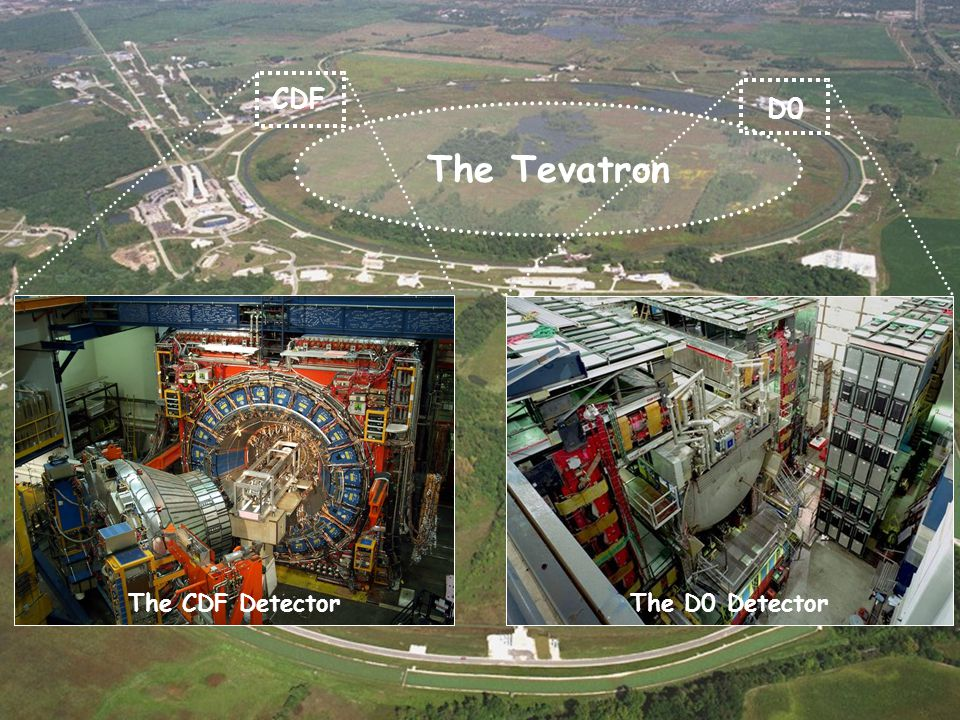
\includegraphics[height=0.5\textheight]{./Images/02_D0_general.jpg}
      \caption*{Aerial view of Fermilab National Accelerator Laboratory}
    \end{figure}
    \itt
  \item[$\Box$] probed $\sqrt{s} = 1.96 TeV$ $p-\bar{p}$ collisions at a rate of
    \alert{$1.2\times 10^{6} s^{-1}$} (\alert{$\approx \mathcal{L}_{int} = 10 fb^{-1}$})
    \tti
  \end{overlayarea}
\end{frame}

%%%%%% SLIDE
\subsection{Experiment goals}

\begin{frame}{\textcolor{Goldenrod}{D$\emptyset$ Experiment Goals}}
  \itt
\item[$\Box$]<1-> \hlt{black}{Precision searches:}
\itt
\item Z and W masses, widths and production cross sections
\item Forward-backward asymmetry
\item $W/Z \to q\bar{q}$
\item $\frac{\alpha_{QCD}}{\alpha_{QED}}$ 
  \tti

\item[$\Box$]<2-> \hlt{Orange}{New physics:}\\
  \itt
\item $Z \to X \gamma; X\to l^+l^-$
\item Single top
\item Gauge boson couplings
\item \hlt{Magenta}{Higgs boson   }
\item \hlt{Red}{Supersymmetry}
\item $W', Z'$, heavy leptons and heavy quarks
\item Surprises !
  \tti
  \tti
\end{frame}  
%%%%% LONG VERSION
% \begin{frame}{\textcolor{Goldenrod}{D$\emptyset$ Experiment Goals}}
% \item[$\Box$] \hlt{black}{Z and W masses:\\}
%   $-$ Z mass from $ Z\to e^+ e^-$ using invariant mass\\
%   $-$ W mass from $W\to l \nu_{l}$ using $m_{T} =
%   \sqrt{2p^{l}_{T}\slashed{E_{T}}(1 - \cos\theta_{l, MET})}$\\
%   $-$ good $\slashed{E_{T}}$ resolution is necessary for $m_T$
% \item[$\Box$] \hlt{black}{Z and W widths:}\\
%   $- $ \alert{$\delta \Gamma_Z = \frac{2}{N} \sqrt{\Gamma^2_Z + (2.35
%       \delta m_Z)^2}$}\\
%   $- $ $\frac{\Gamma_W}{\Gamma_Z}$ within 8\% $\to$ QCD radiative
%   corrections  \& narrowing down $m_t$ mass window

% \item[$\Box$] \hlt{black}{$Z \to X \gamma; X\to l^+l^-$ searches:} \\
%   $- $ electronic to muonic decay ratio is needed\\
%   $- $ \alert{ good $\gamma$ ( ~ 10 GeV) and $\pi^0$ separation is
%     essential}
  
% \item[$\Box$] \hlt{black}{ Forward-backward asymmetry:}\\
%   $- $ $b\bar{b}$ decay was of special interest due to pure measurements
%   from other experiments\\
%   $- $ good muon identification at $p_T \approx 100 GeV/c$
  
% %% 03_tri_couplings  
% \item  \hlt{black}{Gauge boson couplings:\\}
%   $- $ associated production of gauge bosons
%   $- $ $p\bar{p} \to W \gamma X; W \to l \nu$ 

% \item \hlt{black}{ W and Z production:}\\
%   $- $ The x-dependence of W and Z production reveal the parton
%   x-distribution in the same way as in Drell-Yan production.\\
  
%   $- $ The $p_T$ distribution of produced bosons is interesting for a
%   study of radiative processes in QCD

% \item \hlt{black}{$W/Z \to q\bar{q}$:}\\
%   $- $ good hadron energy measurement in order to reduce the error on jet
%   invariant mass.\\
%   $- $ good segmentation of calorimetry is also desired
  
% \item \hlt{black}{ $\frac{\alpha_{QCD}}{\alpha_{QED}}$ :\\} 
%   $- $ single $\gamma$ to single $g$ production 
%   \tti
  
% \end{frame}


\subsection{Design considerations}
%%%%%%%% SLIDE
\begin{frame}{\textcolor{Goldenrod}{D$\emptyset$ Design Considerations}}
  \itt
\item[$\bullet$]<1-> \textcolor{blue}{Electromagnetic energy resolution at the level of $\delta E / E
    = \frac{0.05}{\sqrt{E}}$ with good $\pi^0-e $ separation}
  % {\small
  %   \itt
  % \item good electron ID for narrow massive states searches and
  %   to lower electron-jet faking rate. \\
  % \item good lateral and longitudinal sampling for single $\gamma$
  %   searches with high $p_T$ (\alert{challenging $\pi^0-e $ separation})
  %   \tti
  % }
  
\item[$\bullet$]<1-> \textcolor{blue}{good muon momentum resolution and
    muon ID}
  % {\small
  %   \itt
  % \item muons are less analyzed, but with charge tagging $\to$ ID them even inside
  %   jets which is important for many searches
  %   \tti
  % }
\item[$\bullet$]<2-> \textcolor{Blue}{Hadron energy resolution of about $\delta E / E
    = \frac{0.8}{\sqrt{E}}$:}
  {\small
    \itt
  \item \textcolor{Magenta}{$p^{jet}_T, m^{jet}$, and $\slashed{E_{T}}$ are critically
      dependent upon it.}
    \tti
  }
\item[$\bullet$]<3-> \textcolor{Blue}{Missing transverse energy resolution:}
  {\small 
    \itt
  % \item good hadron energy resolution $\to$ uranium-liquid argon
  %   calorimerty was chosen.
    
  \item \textcolor{Magenta}{angular coverage down to about $1^{\circ}$}
    
  \item minimizing dead areas in the large angle calorimetry
    \tti
  }
  \tti   
\end{frame}

%%%%%% The upgraded D0
\begin{frame}{\textcolor{Goldenrod}{Upgraded D$\emptyset$}}
  \begin{figure}[h]
    \img{00_upgraded_D0}
    \caption*{upgraded D$\emptyset$ detector viewed from inside the Tevatron ring}
  \end{figure}
\end{frame}

%%%%%%% SLIDE 
\begin{frame}{\textcolor{Goldenrod}{Upgraded D$\emptyset$ }}
  % \<{0.5\textwidth}
  % \begin{center}
  %   \img{01_dzero_wholedetector}
  % \end{center}
  % % \caption*{{\scriptsize A simplified cross section view of the
  % % D$\emptyset$   }}
  % \>
  \itt
\item[$\Box$]<only@1> \hlt{Blue}{in 2001 after the Main Injector and associated Tevatron
  upgrades the instantaneous luminosity increased by more than a factor of ten}
  
\item[$\Box$]<only@1> \hlt{Magenta}{The central tracking system was completely replaced.}
  {\small
    \itt
  \item \alert{the old system lacked a magnetic field and suffered from radiation
      damage}
  \item improved tracking technologies are now available.\\
  \item The new system included a silicon microstrip tracker and a
    scintillating-fiber tracker located within a 2 T solenoidal
    magnet.
    \tti
  }
\item[$\Box$]<only@2> \hlt{blue}{Between the solenoidal magnet and the central calorimeter and
    in front of the forward calorimeters, preshower detectors have
    been added for improved electron identification.}
  
\item[$\Box$]<only@2> \hlt{blue}{In the forward muon system, proportional drift chambers are
    replaced by mini drift tubes and trigger scintillation
    counters\\}
  {\small
    \itt
  \item which can withstand the harsh radiation environment and
    additional shielding has been added.
    
  \item \alert{In the central region,
      scintillation counters have been added for improved muon
      triggering.}
    \tti
  }
  \tti
\end{frame}

